\documentclass[a4paper,12pt]{article}
\usepackage{amsmath}
\usepackage{amsfonts}
\usepackage{amssymb}
\usepackage{graphicx}
\usepackage{tikz}
\usepackage{geometry}
\usetikzlibrary{positioning,shapes.geometric}
\geometry{a4paper, margin=1in}
\title{Database Design for Privat Transport}
\author{4060}
\date{\today}
\begin{document}
\maketitle

\section*{Introduction}
This document details the database design process for Privat Transport, a private transport company established in Grimstad in 2023. The design follows a structured methodology comprising conceptual, logical, and physical database design phases. The objective is to create a database application to support the operations of Privat Transport, addressing issues of information sharing and administrative efficiency.

\section*{Conceptual Database Design}
The conceptual database design involves constructing a model of the data requirements independent of physical considerations. The steps include identifying entity types, relationship types, attributes, and keys, and validating the model against user transactions.

\subsection*{Step 1.1: Identify Entity Types}
\begin{itemize}
    \item \textbf{Office}
    \item \textbf{Manager}
    \item \textbf{CarOwner}
    \item \textbf{Driver}
    \item \textbf{AdministrativeStaff}
    \item \textbf{Car}
    \item \textbf{PrivateClient}
    \item \textbf{BusinessClient}
    \item \textbf{Contract}
    \item \textbf{Job}
\end{itemize}

\subsection*{Step 1.2: Identify Relationship Types}
\begin{itemize}
    \item \textbf{Manager Manages Office}
    \item \textbf{CarOwner Owns Car}
    \item \textbf{Driver Drives Car}
    \item \textbf{Office Employs AdministrativeStaff}
    \item \textbf{PrivateClient Requests Job}
    \item \textbf{BusinessClient Has Contract}
    \item \textbf{Contract Includes Job}
    \item \textbf{Job AssignedTo Driver}
    \item \textbf{Job Uses Car}
\end{itemize}

\subsection*{Step 1.3: Identify and Associate Attributes}
\begin{itemize}
    \item \textbf{Office}: officeID, city
    \item \textbf{Manager}: managerID, name, phone, officeID
    \item \textbf{CarOwner}: ownerID, name, phone
    \item \textbf{Driver}: driverID, name, sex, DOB, phone, officeID
    \item \textbf{AdministrativeStaff}: staffID, name, phone, officeID
    \item \textbf{Car}: carID, registrationNo, model, ownerID
    \item \textbf{PrivateClient}: clientID, name, phone, address
    \item \textbf{BusinessClient}: clientID, name, phone, address
    \item \textbf{Contract}: contractID, clientID, numberOfJobs, fee
    \item \textbf{Job}: jobID, clientID, contractID, pickUpDateTime, pickUpAddress, dropOffAddress, mileage, charge, status
\end{itemize}

\subsection*{Step 1.4: Determine Attribute Domains}
\begin{itemize}
    \item \textbf{officeID}: Integer
    \item \textbf{managerID, ownerID, driverID, staffID, clientID, contractID, jobID}: Integer
    \item \textbf{name, phone, address, model, registrationNo}: String
    \item \textbf{sex}: Char (M, F)
    \item \textbf{DOB, pickUpDateTime}: Date
    \item \textbf{numberOfJobs, mileage}: Integer
    \item \textbf{fee, charge}: Decimal
    \item \textbf{status}: String (Completed, Failed)
\end{itemize}

\subsection*{Step 1.5: Determine Candidate, Primary, and Alternate Key Attributes}
\begin{itemize}
    \item \textbf{Office}: Primary Key = officeID
    \item \textbf{Manager}: Primary Key = managerID
    \item \textbf{CarOwner}: Primary Key = ownerID
    \item \textbf{Driver}: Primary Key = driverID
    \item \textbf{AdministrativeStaff}: Primary Key = staffID
    \item \textbf{Car}: Primary Key = carID
    \item \textbf{PrivateClient}: Primary Key = clientID
    \item \textbf{BusinessClient}: Primary Key = clientID
    \item \textbf{Contract}: Primary Key = contractID
    \item \textbf{Job}: Primary Key = jobID
\end{itemize}

\subsection*{Step 1.6: Consider Use of Enhanced Modeling Concepts (Optional)}
\begin{itemize}
    \item Specialization: \textbf{Client} superclass with \textbf{PrivateClient} and \textbf{BusinessClient} subclasses.
\end{itemize}

\subsection*{Step 1.7: Check Model for Redundancy}
\begin{itemize}
    \item Ensure no redundant entities or relationships exist.
\end{itemize}

\subsection*{Step 1.8: Validate Conceptual Model Against User Transactions}
\begin{itemize}
    \item Validate that the model supports all user transactions such as listing managers, female drivers, total staff, car details, etc.
\end{itemize}

\subsection*{Step 1.9: Review Conceptual Data Model with User}
\begin{itemize}
    \item Review the ER diagram and associated documentation with the user.
\end{itemize}

\begin{figure}[!ht]
\centering
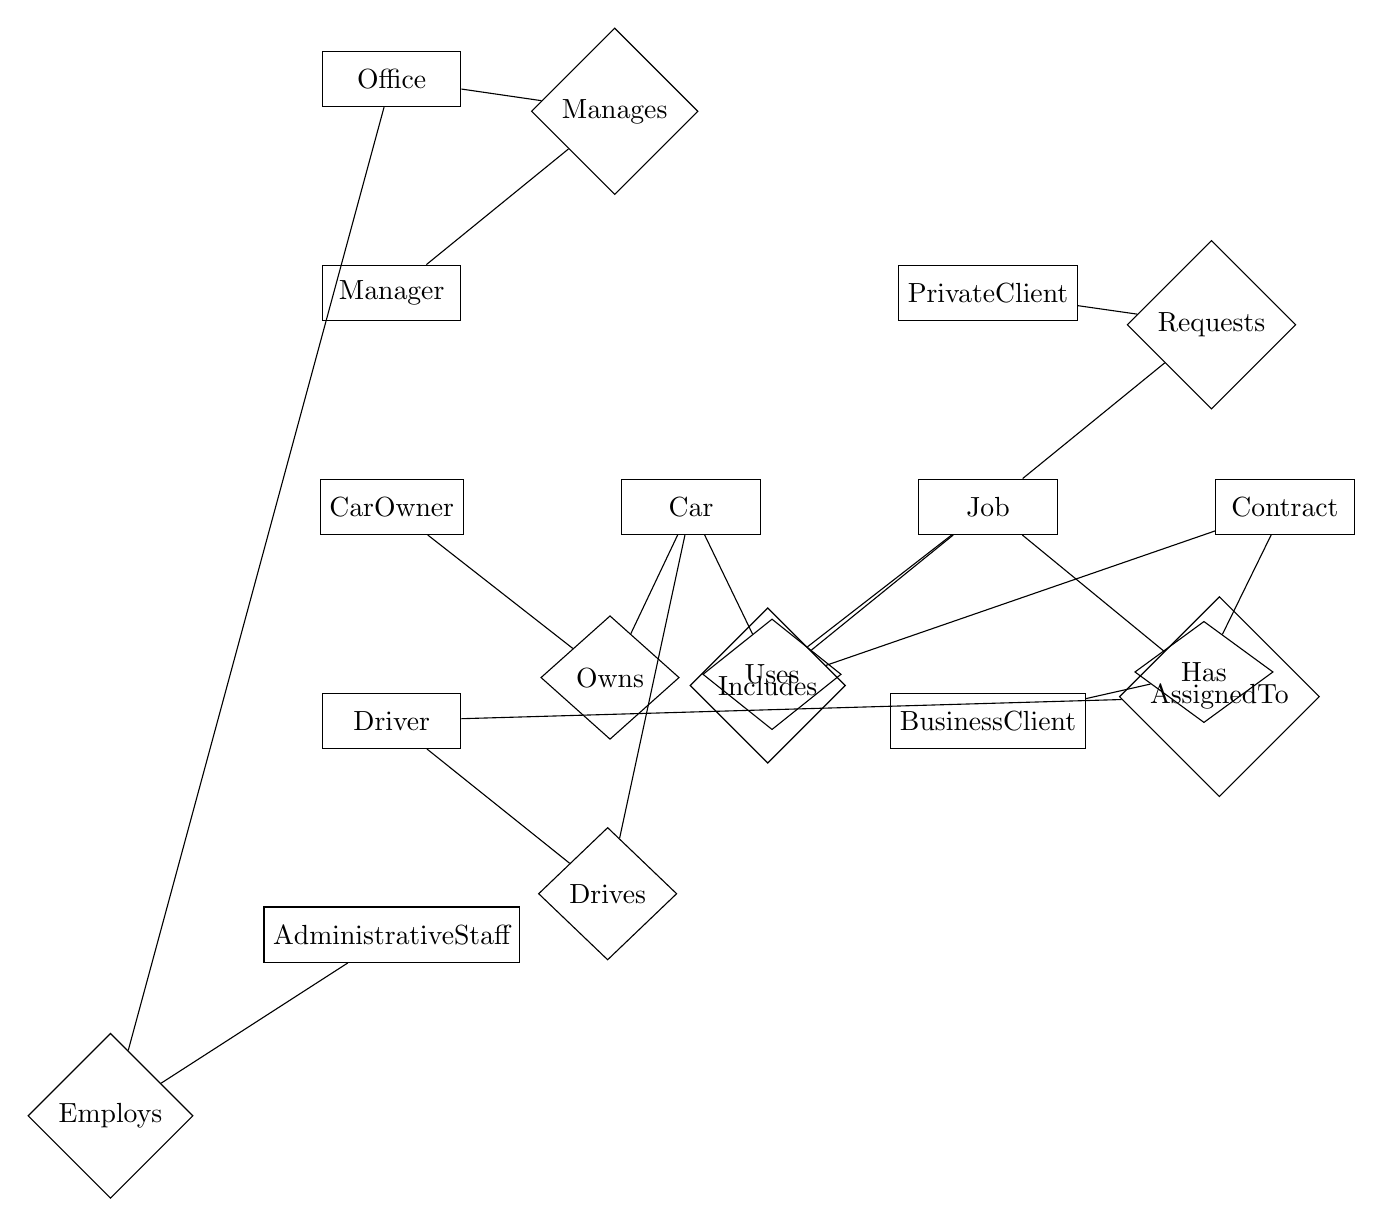
\begin{tikzpicture}[node distance=2cm]
  \tikzset{
    entity/.style={draw, rectangle, minimum height=2em, minimum width=5em, text centered},
    relationship/.style={draw, diamond, minimum height=2em, minimum width=5em, text centered}
  }

  \node[entity] (office) {Office};
  \node[entity, below=of office] (manager) {Manager};
  \node[entity, below=of manager] (owner) {CarOwner};
  \node[entity, below=of owner] (driver) {Driver};
  \node[entity, below=of driver] (staff) {AdministrativeStaff};
  \node[entity, right=of owner] (car) {Car};
  \node[entity, right=of car] (job) {Job};
  \node[entity, above=of job] (pclient) {PrivateClient};
  \node[entity, below=of job] (bclient) {BusinessClient};
  \node[entity, right=of job] (contract) {Contract};

  \node[relationship, above right=of manager] (manages) {Manages};
  \node[relationship, below right=of owner] (owns) {Owns};
  \node[relationship, below right=of driver] (drives) {Drives};
  \node[relationship, below left=of staff] (employs) {Employs};
  \node[relationship, above right=of job] (requests) {Requests};
  \node[relationship, below right=of job] (has) {Has};
  \node[relationship, below left=of job] (includes) {Includes};
  \node[relationship, below right=of job] (assignedto) {AssignedTo};
  \node[relationship, below left=of job] (uses) {Uses};

  \draw (office) -- (manages);
  \draw (manages) -- (manager);
  \draw (owner) -- (owns);
  \draw (owns) -- (car);
  \draw (driver) -- (drives);
  \draw (drives) -- (car);
  \draw (office) -- (employs);
  \draw (employs) -- (staff);
  \draw (pclient) -- (requests);
  \draw (requests) -- (job);
  \draw (bclient) -- (has);
  \draw (has) -- (contract);
  \draw (contract) -- (includes);
  \draw (includes) -- (job);
  \draw (job) -- (assignedto);
  \draw (assignedto) -- (driver);
  \draw (job) -- (uses);
  \draw (uses) -- (car);
\end{tikzpicture}
\caption{ER Diagram for Privat Transport}
\end{figure}

\newpage

\section*{Logical Database Design}
The logical database design translates the conceptual data model into a relational model. The steps include deriving relations, validating them using normalization, and ensuring they support user transactions.

\subsection*{Step 2.1: Derive Relations for Logical Data Model}
\begin{itemize}
    \item \textbf{Office(officeID, city)}
    \item \textbf{Manager(managerID, name, phone, officeID)}
    \item \textbf{CarOwner(ownerID, name, phone)}
    \item \textbf{Driver(driverID, name, sex, DOB, phone, officeID)}
    \item \textbf{AdministrativeStaff(staffID, name, phone, officeID)}
    \item \textbf{Car(carID, registrationNo, model, ownerID)}
    \item \textbf{PrivateClient(clientID, name, phone, address)}
    \item \textbf{BusinessClient(clientID, name, phone, address)}
    \item \textbf{Contract(contractID, clientID, numberOfJobs, fee)}
    \item \textbf{Job(jobID, clientID, contractID, pickUpDateTime, pickUpAddress, dropOffAddress, mileage, charge, status)}
\end{itemize}

\subsection*{Step 2.2: Validate Relations Using Normalization}
Ensure all relations are in at least Third Normal Form (3NF) to eliminate redundancy and ensure data integrity.

\subsection*{Step 2.3: Validate Relations Against User Transactions}
Check that each relation supports the necessary user transactions.

\subsection*{Step 2.4: Define Integrity Constraints}
Ensure all primary keys, foreign keys, and other constraints are correctly defined.

\subsection*{Step 2.5: Review Logical Data Model with User}
Review the logical data model with the user for accuracy and completeness.

\begin{figure}[!ht]
\centering
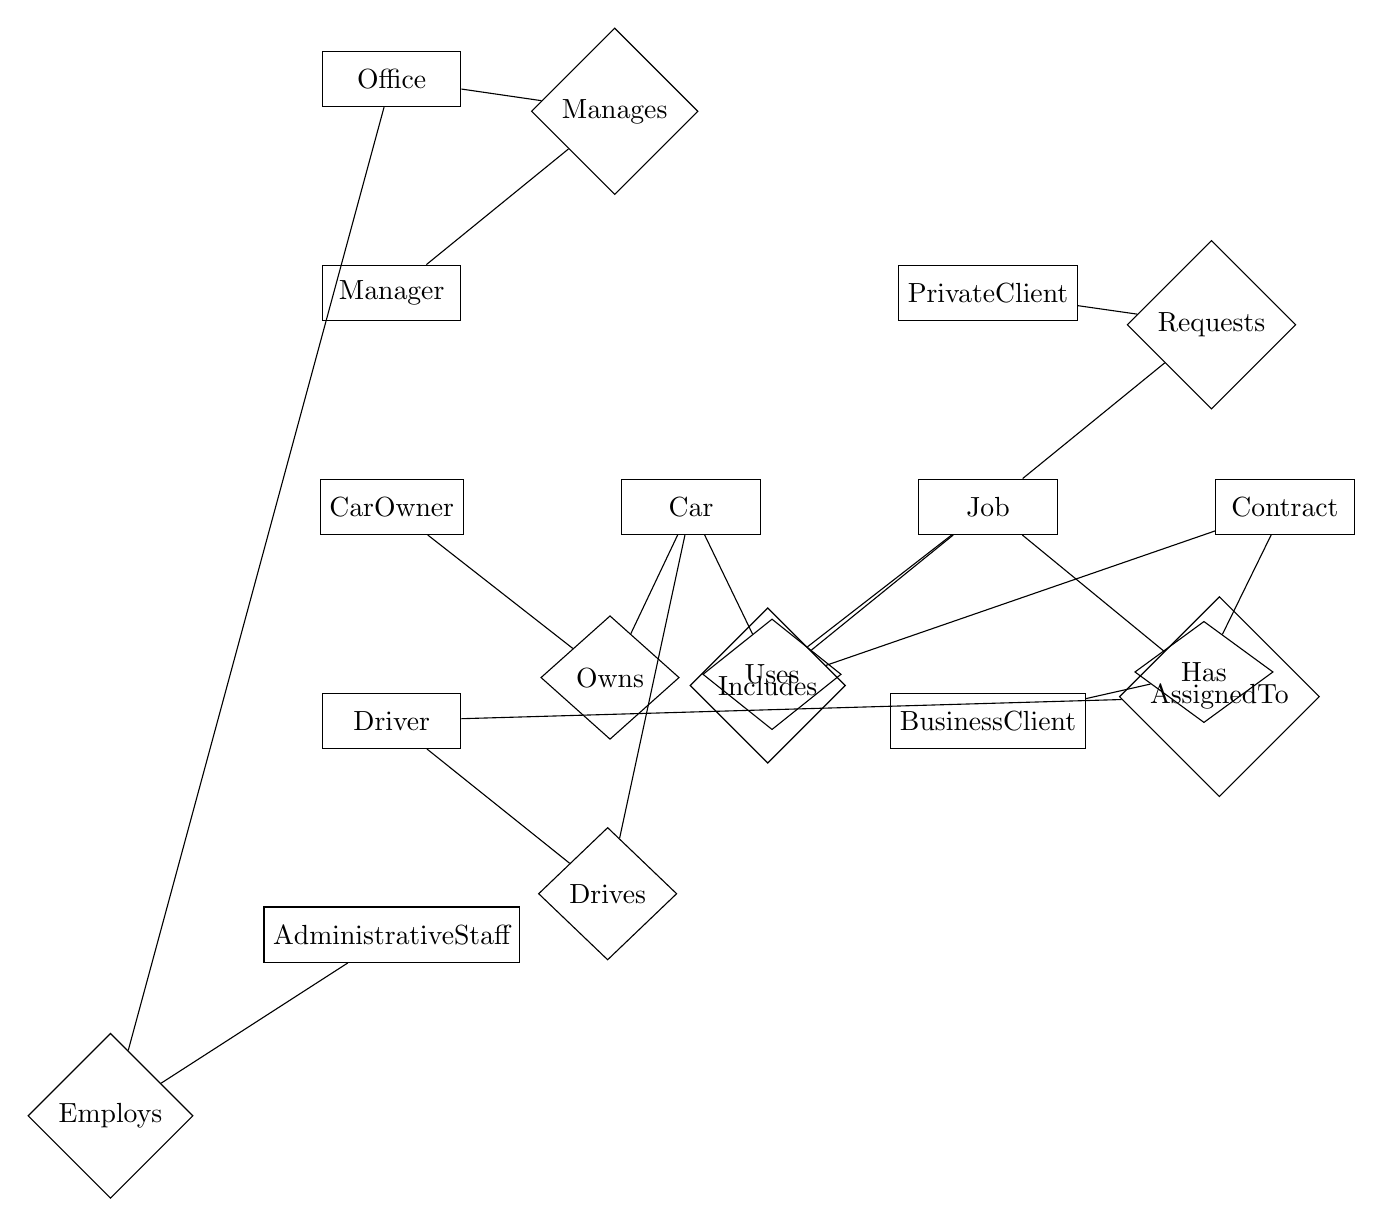
\begin{tikzpicture}[node distance=2cm]
  \tikzset{
    entity/.style={draw, rectangle, minimum height=2em, minimum width=5em, text centered},
    relationship/.style={draw, diamond, minimum height=2em, minimum width=5em, text centered}
  }

  \node[entity] (office) {Office};
  \node[entity, below=of office] (manager) {Manager};
  \node[entity, below=of manager] (owner) {CarOwner};
  \node[entity, below=of owner] (driver) {Driver};
  \node[entity, below=of driver] (staff) {AdministrativeStaff};
  \node[entity, right=of owner] (car) {Car};
  \node[entity, right=of car] (job) {Job};
  \node[entity, above=of job] (pclient) {PrivateClient};
  \node[entity, below=of job] (bclient) {BusinessClient};
  \node[entity, right=of job] (contract) {Contract};

  \node[relationship, above right=of manager] (manages) {Manages};
  \node[relationship, below right=of owner] (owns) {Owns};
  \node[relationship, below right=of driver] (drives) {Drives};
  \node[relationship, below left=of staff] (employs) {Employs};
  \node[relationship, above right=of job] (requests) {Requests};
  \node[relationship, below right=of job] (has) {Has};
  \node[relationship, below left=of job] (includes) {Includes};
  \node[relationship, below right=of job] (assignedto) {AssignedTo};
  \node[relationship, below left=of job] (uses) {Uses};

  \draw (office) -- (manages);
  \draw (manages) -- (manager);
  \draw (owner) -- (owns);
  \draw (owns) -- (car);
  \draw (driver) -- (drives);
  \draw (drives) -- (car);
  \draw (office) -- (employs);
  \draw (employs) -- (staff);
  \draw (pclient) -- (requests);
  \draw (requests) -- (job);
  \draw (bclient) -- (has);
  \draw (has) -- (contract);
  \draw (contract) -- (includes);
  \draw (includes) -- (job);
  \draw (job) -- (assignedto);
  \draw (assignedto) -- (driver);
  \draw (job) -- (uses);
  \draw (uses) -- (car);
\end{tikzpicture}
\caption{ER Diagram for Logical Data Model}
\end{figure}

\newpage

\section*{Physical Database Design}
The physical database design involves translating the logical data model into a physical implementation on MySQL. This includes defining the SQL schema and constraints.

\subsection*{Step 3.1: Translate Logical Data Model for MySQL}
Create SQL scripts for each table based on the logical data model.

\subsection*{SQL Implementation}

\subsubsection*{Create Tables}
\begin{verbatim}
CREATE TABLE Office (
    officeID INT PRIMARY KEY,
    city VARCHAR(100)
);

CREATE TABLE Manager (
    managerID INT PRIMARY KEY,
    name VARCHAR(100),
    phone VARCHAR(15),
    officeID INT,
    FOREIGN KEY (officeID) REFERENCES Office(officeID)
);

CREATE TABLE CarOwner (
    ownerID INT PRIMARY KEY,
    name VARCHAR(100),
    phone VARCHAR(15)
);

CREATE TABLE Driver (
    driverID INT PRIMARY KEY,
    name VARCHAR(100),
    sex CHAR(1),
    DOB DATE,
    phone VARCHAR(15),
    officeID INT,
    FOREIGN KEY (officeID) REFERENCES Office(officeID)
);

CREATE TABLE AdministrativeStaff (
    staffID INT PRIMARY KEY,
    name VARCHAR(100),
    phone VARCHAR(15),
    officeID INT,
    FOREIGN KEY (officeID) REFERENCES Office(officeID)
);

CREATE TABLE Car (
    carID INT PRIMARY KEY,
    registrationNo VARCHAR(10),
    model VARCHAR(50),
    ownerID INT,
    FOREIGN KEY (ownerID) REFERENCES CarOwner(ownerID)
);

CREATE TABLE PrivateClient (
    clientID INT PRIMARY KEY,
    name VARCHAR(100),
    phone VARCHAR(15),
    address VARCHAR(255)
);

CREATE TABLE BusinessClient (
    clientID INT PRIMARY KEY,
    name VARCHAR(100),
    phone VARCHAR(15),
    address VARCHAR(255)
);

CREATE TABLE Contract (
    contractID INT PRIMARY KEY,
    clientID INT,
    numberOfJobs INT,
    fee DECIMAL(10,2),
    FOREIGN KEY (clientID) REFERENCES BusinessClient(clientID)
);

CREATE TABLE Job (
    jobID INT PRIMARY KEY,
    clientID INT,
    contractID INT,
    pickUpDateTime DATETIME,
    pickUpAddress VARCHAR(255),
    dropOffAddress VARCHAR(255),
    mileage INT,
    charge DECIMAL(10,2),
    status VARCHAR(20),
    FOREIGN KEY (clientID) REFERENCES PrivateClient(clientID),
    FOREIGN KEY (contractID) REFERENCES Contract(contractID)
);
\end{verbatim}

\section*{Conclusion}
This document presents the complete database design process for Privat Transport, including conceptual, logical, and physical design phases. The models and SQL scripts provided ensure a robust database implementation suitable for the company's needs.

\end{document}
